% !TeX spellcheck = cs_CZ
%{\tikzset{external/prefix={tikz/FYZI/}}
% \tikzset{external/figure name/.add={ch07_}{}}
%---------------------------------------------------------------------------------------------------
% file fey1ch09.tex
%---------------------------------------------------------------------------------------------------
%================ Kapitola: Newtonovy zákony dynamiky =============================================
\setchaptertoc
\chapter{Newtonovy zákony dynamiky}\label{fyz:IchapIX}

  \section{Hybnost a síla}\label{fyz:IchapIXsecI}
    Objev zákonů dynamiky neboli zákonů pohybu, byl dramatickým momentem v historii vědy. Ještě 
    před Newtonem byly pohyby takových objektů, jako jsou planety, záhadou, ale po Newtonovi se 
    stalo vše pochopitelným. Dokonce bylo možné spočítat i malé odchylky od Keplerových zákonů 
    podmiňované působením jiných planet. Po Newtonově objevu bylo možné plně analyzovat pohyb 
    kyvadla, kmity závaží zavěšeného na pružině a jiné jevy. Tak je to i s touto kapitolou: před ní 
    jsme neuměli vypočítat, jak se pohybuje závaží upevněné na pružině a tím méně vypočítat vliv 
    Jupiteru a Saturnu na pohyb Uranu. Po této kapitole budeme schopni vypočítat nejen pohyb 
    kmitajícího závaží, ale i poruchy pohybu Uranu způsobované Jupiterem a Saturnem!
    
    Galileo udělal veliký krok na cestě za pochopením pohybu svým objevem \textbf{principu 
    setrvačnosti}: \emph{Je-li předmět ponechán sám sobě bez vnějších vlivů, pokračuje v přímočarém 
    pohybu konstantní rychlostí, jak se původně pohyboval, nebo zůstává nehybný, jak původně stál.} 
    Taková situace se samozřejmě nikdy neobjevuje v přírodě a postrčíme-li předmět na stole, 
    zastaví se. Zastaví se proto, že nebyl ponechán sám sobě - tře se totiž o stůl. Nalezení tohoto 
    zákona vyžadovalo značnou představivost a tu měl právě Galileo.
    
    Abychom se však dostali dále, musíme znát zákon, podle něhož předměty \emph{mění} svou 
    rychlost, jestliže \emph{jsou} něčím ovlivňovány. To udělal Newton. Newton zformuloval tři 
    zákony. První zákon byl jen opakováním uvedeného Galileova principu setrvačnosti. Druhý zákon 
    určuje, jak se mění rychlost v důsledku různých vlivů nazývaných \textbf{silami}. Třetí zákon 
    do určité míry popisuje síly, ale o tomto zákoně budeme hovořit jindy. Nyní si budeme všímat 
    Newtonova druhého pohybového zákona, který udává, jak síla ovlivňuje pohyb nějakého objektu a 
    říká, že \emph{změna veličiny zvané hybnost za jednotku času je úměrná síle}. Později toto 
    tvrzení stručné matematicky zapíšeme, ale nejprve vysvětlíme jeho podstatu.
    
    \textbf{Hybnost} není totéž, co rychlost Ve fyzice používáme mnoho slov a každé z nich má 
    přesný význam, ačkoli v každodenní běžné řeči se takováto přesnost nevyžaduje. Nyní se 
    zamysleme nad definicí hybnosti. Zatlačíme-li rukou na nějaký lehký předmět, snadno ho uvedeme 
    do pohybu. Zatlačíme-li stejně na mnohem těžší předmět, bude se pohybovat mnohem pomaleji. 
    Namísto slov „lehký“ a „těžký“ však musíme používat výrazy s \emph{menší hmotností} a 
    \emph{větší hmotnosti} neboť mezi tíhou a setrvačností předmětu je rozdíl, který musíme brát v 
    úvahu. (Jak těžké je uvést předmět do pohybu a jakou má tíhu, to jsou dvě rozdílné věci.) Tíha 
    a setrvačnost jsou \emph{úměrné} a na zemském povrchu je často považujeme za číselně stejné, a 
    právě to vyvolává u některých studentů rozpaky. \emph{Na Marsu by se tíha předmětů lišila od 
    jejich tíhy na Zemi, ale množství síly potřebné na překonání setrvačnosti by se nezměnilo}.
    
    Termín \textbf{hmotnost} používáme jako \textbf{kvantitativní míru setrvačnosti}. Hmotnost 
    můžeme měřit například tak, že zavěšeným předmětem budeme kroužit určitou rychlostí a budeme 
    měřit sílu, která je potřebná k jeho udržení v otáčivém pohybu. Takovýmto způsobem můžeme 
    každému předmětu přisoudit určitou hmotnost. \emph{Hybnost} předmětu je součinem dvou faktorů: 
    jeho \emph{hmotnosti} a jeho \emph{rychlosti}. Druhý Newtonův zákon je proto možné zapsat v 
    matematickém tvaru
    \begin{equation}\label{fyz:eq052}
      \vec{F} = \der{}{t}(m\vec{v}).
    \end{equation}
    
    K tomu je třeba uvést několik poznámek. Při zápisu takového zákona se opíráme o mnoho 
    intuitivních myšlenek, náznaků a předpokladů, jež v prvním stádiu zkombinujeme přibližně do 
    našeho „zákona“. Později se můžeme vrátit zpět a detailně zvážit význam každého členu. 
    Pokusíme-li se však o to příliš brzy, můžeme se dostat do rozpaků. Proto budeme pro začátek 
    považovat některé věci za samozřejmé. Budeme předpokládat, že hmotnost předmětu je 
    \emph{konstantní}. Hmotnost ve skutečnosti konstantní není, ale začneme s Newtonovou aproximací 
    konstantní, po celou dobu neměnné hmotnosti a dále budeme předpokládat, že předmět vytvořený 
    složením dvou předmětů má hmotnost rovnou součtu jejich hmotností. Newton při sestavování své 
    rovnice z těchto předpokladů vycházel, vždyť jinak by jeho rovnice neměla smysl. Představme si 
    třeba, že hmotnost se mění nepřímo úměrně rychlosti. Pak by se hybnost za \emph{žádných 
    okolností neměnila}. Zákon má smysl jen tehdy, když víme, jak se hmotnost mění s rychlostí. 
    Proto zatím předpokládáme, že hmotnost se \emph{nemění}.
    
    Dále si musíme podrobněji všimnout \emph{síly}. V hrubé představě ji považujeme za zatlačení 
    nebo zatáhnutí, které provedou naše svaly, ale když máme k dispozici pohybový zákon, můžeme 
    sílu definovat přesněji. Nejdůležitější co si musíme uvědomit, je skutečnost, že tento zákon 
    nezahrnuje jen změny velikosti hybnosti nebo rychlosti, ale i změny jejich \emph{směru}. Je-li 
    hmotnost konstantní, rovnici (\ref{fyz:eq052}) je možné napsat ve tvaru
    \begin{equation}\label{fyz:eq053}
      \boxed{
        \vec{F} = m\der{\vec{v}}{t} = m\vec{a}.
       }
    \end{equation}
    
    \textbf{Zrychlení} a představuje změnu rychlosti za jednotku času a Newtonův druhý pohybový 
    zákon říká více než to, že účinek síly se mění nepřímo úměrně hmotnosti. Říká i, že směr změny 
    rychlosti a směr síly jsou shodné. Proto si musíme uvědomit, že změna rychlosti, neboli 
    zrychlení, má širší význam než v hovorové řeči. Rychlost pohybujícího se předmětu se může měnit 
    tak, že se jeho pohyb zrychluje, zpomaluje, nebo se mění směr pohybu. Zrychlení kolmé na směr 
    rychlosti jsme uvažovali v kapitole \ref{fyz:chap_fey_gravity}. Tam jsme viděli, že předmět 
    pohybující se po kružnici s poloměrem \(R\) rychlostí \(v\) se vychyluje od přímočaré dráhy o 
    vzdálenost \(\frac{1}{2}\frac{v^2}{R}t\), je-li \(t\) velmi malé. Proto vztah pro zrychlení 
    kolmé na směr pohybuje
    \begin{equation}\label{fyz:eq059}
      a = \frac{v^2}{R}.
    \end{equation}
    
    Síla působící ve směru kolmém k rychlosti vyvolá proto pohyb předmětu po zakřivené dráze, jejíž 
    poloměr křivosti můžeme získat tak, že sílu dělíme hmotností předmětu (tak dostaneme zrychlení) 
    a pak použijeme vztah (\ref{fyz:eq059}).
    
  \section{Směr a velikost rychlosti}\label{fyz:IchapIXsecII}
    Abychom upřesnili náš jazyk, musíme se hlouběji zamyslet nad pojmem rychlost V hovorové řeči se 
    se slovem rychlost setkáváme často. Takto používaný pojem má však chudší obsah než pojem 
    \emph{rychlost} používaný ve fyzice.

    \begin{figure}[ht!]  %\ref{fyz:fig056}
      \centering
      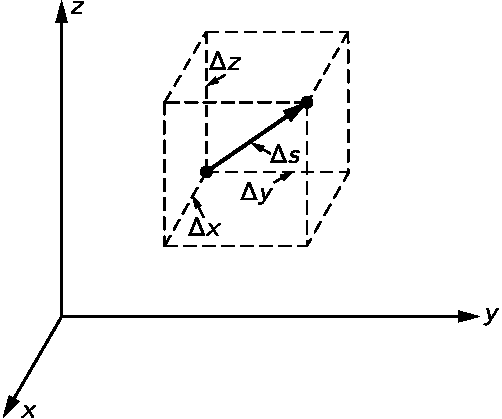
\includegraphics[width=0.6\linewidth]{fyz_fig056.pdf}
      \caption{Malé posunutí předmětu (\cite[s.~124]{Feynman01})}
      \label{fyz:fig056}
    \end{figure}
    
    Rychlost jako fyzikální veličina znamená určitou velikost, tj. jistý počet metrů za sekundu, 
    ale i směr, v němž se uskutečňuje pohyb, zatímco v hovorové řeči znamená jen velikost. 
    Matematicky můžeme vystihnout velikost i směr rychlosti, určíme-li, jak se souřadnice \emph{x, 
    y, z} daného předmětu mění s časem. Nechť se například v určitém časovém okamžiku předmět 
    pohybuje tak, jak je znázorněno na obr. \ref{fyz:fig056}. V malém časovém intervalu \(\Delta 
    t\) urazí jistou vzdálenost \(\Delta x\) ve směru osy \(x\), \(\Delta y\) ve směru \(y\) a 
    \(\Delta z\) ve směru osy \(z\). Výsledkem těchto tří změn souřadnic je posunutí \(\Delta s\) 
    podél úhlopříčky rovnoběžnostěnu se stranami \(\Delta x\), \(\Delta y\), \(\Delta z\). Posunutí 
    \(\Delta x\) je součin x-ové složky rychlosti a intervalu \(\Delta t\) a podobné vztahy platí 
    pro \(\Delta y\), \(\Delta z\)
    \begin{equation}\label{fyz:eq060}
      \Delta x = v_x\Delta t,\quad \Delta y = v_y\Delta t,\quad \Delta z = v_z\Delta t.
    \end{equation}
    
  \section{Složky rychlosti, zrychlení a síly}\label{fyz:IchapIXsecIII}
    Vztah (\ref{fyz:eq060}) představuje rozklad rychlostí na složky, které nám udávají, jak rychle 
    se předmět pohybuje ve směru osy \(x\), \(y\), a \(z\). Velikost i směr rychlosti budou plně 
    určeny, udáme-li číselné hodnoty jejich tří kolmých složek
    \begin{equation}\label{fyz:eq061}
      v_x = \der{x}{t}, v_y = \der{y}{t}, v_z = \der{z}{t}
    \end{equation}

    \begin{figure}[ht!]  %\ref{fyz:fig057}
      \centering
      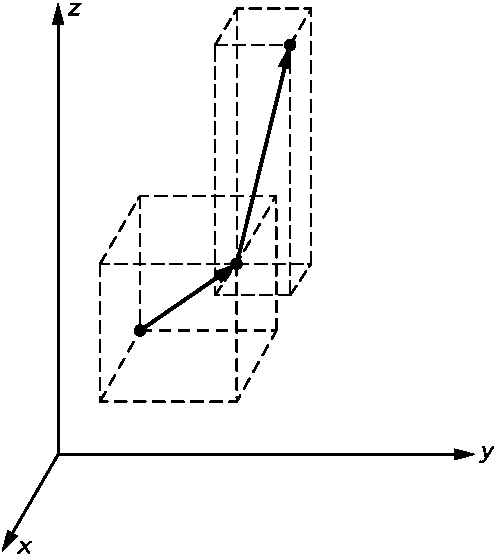
\includegraphics[width=0.5\linewidth]{fyz_fig057.pdf}
      \caption{Změna rychlosti, při níž se mění její velikost i směr (\cite[s.~125]{Feynman01})}
      \label{fyz:fig057}
    \end{figure}
    
    Přitom velikost rychlosti předmětu je
    \begin{equation}\label{fyz:eq062}
      \der{s}{t} = \abs{v} = \sqrt{v^2_x + v^2_y + v^2_z}. 
    \end{equation}
    
    Nyní předpokládejme, že působením síly mění rychlost svůj směr a velikost tak, jak je to 
    znázorněno na obr. \ref{fyz:fig057}. Tuto zdánlivě složitou situaci vyřešíme poměrně snadno, 
    určíme-li změny složek rychlosti. Změna složky rychlosti ve směru osy \(x\) za čas \(\Delta t\) 
    je \(\Delta v_x = a_x\Delta t\), přičemž \(a_x\) je x-ová složka zrychlení. Podobně je \(\Delta 
    v_y = a_y\Delta t\), \(\Delta v_z = a_z\Delta t\). Vidíme, že Newtonův druhý pohybový 
    zákon tím, že hovoří o shodnosti směru síly a zrychlení, představuje vlastně tři zákony. Každá 
    ze složek síly ve směrech \(x, y, z\) je totiž rovna součinu hmotnosti a časové změny 
    odpovídající složky rychlosti.
    \begin{subequations}\label{fyz:eq063}
      \begin{align}
        F_x &= m\der{v_x}{t} = m\dder{x}{t} = ma_x, \\
        F_y &= m\der{v_y}{t} = m\dder{y}{t} = ma_y, \\
        F_z &= m\der{v_z}{t} = m\dder{z}{t} = ma_z. 
      \end{align}
    \end{subequations}
    
    Podobně jako rychlost a zrychlení je možné i sílu rozložit na složky promítnutím úsečky rovné 
    absolutní hodnotě síly a ukazující směr působení síly na souřadnicové osy \(x, y, z\):
    \begin{subequations}\label{fyz:eq064}
      \begin{align}
        F_x &= F\cos(x,F),\\
        F_y &= F\cos(y,F),\\
        F_z &= F\cos(z,F).
      \end{align}
    \end{subequations}

    Pod \(F\) rozumíme velikost síly a \((x, F)\) představuje úhel, jenž svírá osa \(x\) se směrem 
    síly atd.
    
    Rovnice (\ref{fyz:eq063}) představují úplnou podobu Newtonova druhého pohybového zákona. 
    Známe-li síly působící na předmět a rozložíme je na jednotlivé složky, můžeme z těchto rovnic 
    určit pohyb předmětu. Uvažujme jednoduchý příklad. Nechť ve směrech \(y\) a \(z\) nepůsobí 
    síly. Jediná síla nechť působí například vertikálně ve směru osy \(x\). Vztah (\ref{fyz:eq063}) 
    říká, že rychlost se bude měnit jen ve vertikálním směru a v horizontálním směru bude zůstávat 
    stálá. To jsme již viděli v případě speciálního zařízení z kapitoly \ref{fyz:chap_fey_gravity} 
    (obr. \ref{fyz:fig058}). Padající těleso se pohybuje tak, že jeho horizontální pohyb se nemění 
    a ve vertikálním směru se pohyb uskutečňuje tak, jako kdyby horizontální pohyb neexistoval. 
    Jinak řečeno, pohyby ve směrech \(x\), \(y\), \(z\) jsou nezávislé, jsou-li složky sil vzájemně 
    nezávislé.
    
  \section{Co je to síla?}\label{fyz:IchapIXsecIV}
    Chceme-li využít Newtonovy zákony, musíme znát matematické vyjádření síly; Newtonovy zákony 
    totiž takříkajíc \emph{zaměřují naši pozornost na síly}. Pohybuje-li se předmět zrychleně, musí 
    na něj něco působit a my musíme toto působení odhalit. Naším budoucím programem v dynamice bude 
    \emph{hledání zákonů platných pro síly}. Sám Newton nám poskytl několik příkladů. Objevil zákon 
    síly všeobecné gravitace. V případě jiných sil nám poskytl alespoň částečnou informaci 
    prostřednictvím svého třetího zákona, který budeme studovat v další kapitole a který hovoří o 
    rovnosti akce a reakce.
    
    Rozšiřme náš předcházející příklad a zajímejme se o síly působící na předmět v blízkosti 
    zemského povrchu. U Země je síla ve vertikálním směru, způsobovaná přitažlivostí, úměrná 
    hmotnosti předmětu a je téměř nezávislá na výšce, jde-li o výšky malé ve srovnání se zemským 
    poloměrem \(R\). Tato síla je rovna \(F= \kappa mM/R^2 = mg\), kde \(g = \kappa M/R^2\) se 
    nazývá \textbf{gravitační zrychlení}. Gravitační zákon nám tedy říká, že tíha je úměrná 
    hmotnosti; tato síla má vertikální směr a je rovna součinu hmotnosti a gravitačního zrychlení. 
    Opět zjišťujeme, že v horizontálním směru jde o pohyb s konstantní rychlostí. Zajímavým pohybem 
    je právě pohyb ve vertikálním směru a pro tento pohyb vyplývá z druhého Newtonova zákona
    \begin{equation}\label{fyz:eq126}
      mg=\left(\dder{x}{t}\right).
    \end{equation}
    
    \luagraphic[0.8]{fyz_fig101.pdf}{Závaží na pružině (\cite[s.~127]{Feynman01})}{fyz:fig101}

    Vykrátíme-li \(m\), zjistíme, že zrychlení ve směru \(x\) je konstantní a je rovno \(g\). To je 
    známý zákon volného pádu pod vlivem gravitace, který vyjadřují rovnice
    \begin{align}
      v_x &= v_0 + gt                       \nonumber \\
        x &= x_0 + v_0t + \frac{1}{2}gt^2.  \label{fyz:eq127}
    \end{align}
    
    Nyní si všimněme dalšího příkladu. Předpokládejme, že jsme sami schopni zkonstruovat zařízení na
    obr. \ref{fyz:fig101}, jež vyvolává sílu úměrnou výchylce od rovnováhy a směřující proti této 
    výchylce. Takovým zařízením je \emph{pružina}. Nebudeme si všímat gravitace, jež je 
    vykompenzována počátečním napnutím pružiny, ale budeme se zajímat jen o \emph{nadbytečné} síly. 
    Pak zjistíme, že taháme-li závaží směrem dolů, pružina ho zvedá, a tlačíme-li závaží nahoru, 
    pružina ho tlačí dolů. Zařízení bylo pečlivě navrženo tak, aby síla byla tím větší, čím více 
    stlačíme závaží nahoru, a to přesně přímo úměrně výchylce od rovnovážné polohy, a podobně 
    nahoru působící síla je úměrná našemu vychýlení závaží směrem dolů. Při sledování dynamiky 
    tohoto zařízení vidíme zajímavý pohyb: nahoru, dolů, nahoru, dolů... Vzniká otázka, zda 
    Newtonovy rovnice popisují tento pohyb správně. Zkusme přesně vypočítat takovýto periodický 
    pohyb pomocí Newtonova zákona (\ref{fyz:eq063}). V našem případě máme
    \begin{equation}\label{fyz:eq128}
      -kx = m\left(\der{v_x}{t}\right).
    \end{equation}
    Jde o situaci, kdy se rychlost ve směru osy \(x\) mění úměrně výchylce \(x\). Nemá smysl teď 
    pracovat s tolika konstantami, a tak si situaci zjednodušíme předpokladem, že se buď změnilo 
    časové měřítko, nebo se změnily jiné jednotky, takže shodou okolností \(k/m = 1\). Pak dostaneme
    \begin{equation}\label{fyz:eq129}
      \der{v_x}{t} = -x.
    \end{equation}
    Abychom mohli pokračovat, musíme zjistit, co je to \(v_x\); jenže my už víme, že je to rychlost 
    změny polohy v čase.
    
  \section{Smysl dynamických rovnic}\label{fyz:IchapIXsecV}
    Pokusme se nyní zjistit, co znamená rovnice (\ref{fyz:eq129}). Nechť v daném časovém okamžiku 
    \(t\) má předmět určitou rychlost \(v\) a polohu \(x\). Jaká bude jeho rychlost a poloha v 
    trochu pozdějším okamžiku \(t+\varepsilon\)? Dokážeme-li odpovědět na tuto otázku, vyřešíme náš 
    problém, neboť vycházíme-li z daných počátečních podmínek, dokážeme určit změny v prvním 
    okamžiku, pak v dalším a dalším a postupně určíme celý vývoj pohybu. Kvůli konkrétnosti 
    předpokládejme, že v čase \(t = 0\) je \(x= 1\) a \(v_x = 0\). Proč se předmět vůbec pohybuje? 
    Protože na něj v kterékoli poloze s výjimkou \(x=0\) působí síla. Je-li \(x > 0\), působí síla 
    směrem nahoru. Proto rychlost, která byla zpočátku nulová, se bude v souladu s pohybovým 
    zákonem měnit. Jakmile začne rychlost růst, předmět se začíná pohybovat nahoru. V libovolném 
    časovém okamžiku \(t\) můžeme při velmi malém \(\varepsilon\) vyjádřit polohu v čase \(t + 
    \varepsilon\) pomocí polohy a rychlosti v čase \(t\) s dostatečnou přesností následujícím 
    způsobem
    \begin{equation}\label{fyz:eq130}
      x(t+\varepsilon) = x(t) + \varepsilon v_x(t).
    \end{equation}
    
    Čím je \(\varepsilon\) menší, tím přesnější je tento výraz, ale i tehdy, kdy \(\varepsilon\) 
    není zanedbatelně malé, je tento výraz ještě přijatelně přesný. Co je možné nyní říci o 
    rychlosti? Abychom mohli stanovit rychlost v čase \(t + \varepsilon\) musíme zjistit, jak se 
    rychlost mění, tj. musíme zjistit \emph{zrychlení}. Jak najdeme zrychlení? V tom nám pomohou 
    zákony dynamiky. Podle nich je zrychlení v naší úloze rovno \(-x\)\footnote{V námi zvolených 
    jednotkách.}. Proto
    \begin{subequations}
      \label{fyz:eq131} 
      \begin{align}
        v_x(t+\varepsilon) &= v_x(t) + \varepsilon a_x(t)  \label{fyz:eq131a}        \\
                           &= v_x(t) - \varepsilon x(t)    \label{fyz:eq131b}
      \end{align}
    \end{subequations} 
    
    Rovnice (\ref{fyz:eq131a}) je jen \emph{kinematická} a říká, že rychlost se mění v důsledku 
    přítomnosti zrychlení. Rovnice (\ref{fyz:eq131b}) je však \emph{dynamická}, neboť dává do 
    souvislosti zrychlení a sílu. Poukazuje na to, že v daném časovém okamžiku můžeme v naší 
    konkrétní úloze nahradit zrychlení výrazem \(-x(t)\). Známe-li tedy v daném čase \(x\) i \(v\), 
    známe i zrychlení, jež nám umožní určit novou rychlost a novou polohu. Takto pracuje 
    \emph{dynamický mechanizmus}. Rychlost se trochu změní v důsledku působení síly a i poloha se 
    trochu změní v důsledku rychlosti.
     
  \section{Numerické řešení rovnic}\label{fyz:IchapIXsecVI}
    Pusťme se nyní do skutečného řešení naší úlohy. Zvolíme třeba \(\varepsilon = \num{0.100}\) 
    sekundy. Provedeme-li všechny výpočty a uvidíme, že \(\varepsilon\) nebylo dost malé, můžeme se 
    vrátit a výpočty provádět s \(\varepsilon = \SI{0.010}{\s}\). Ptáme se, jaké je 
    \(x(\num{0.1})\), vycházíme-li z počáteční hodnoty \(x(0) = \num{1.00}\). Bude rovno původní 
    poloze \(x(0)\) zvětšené o rychlost (která je nulová) násobenou \SI{0.10}{\s}. Proto je 
    \(x(0,1)\) stále rovno \num{1.00}, neboť pohyb ještě nezačal. Nová rychlost v čase 
    \SI{0.10}{\s} bude rovna původní rychlosti \(v(0) = 0\) zvětšené o součin \(\varepsilon\) a 
    zrychlení. Zrychlení je \(-x(0) = \num{-1.00}\). Je tedy
    \begin{align*}
      v(\num{0.1}) &= \num{0.00} - \num{0.10}\cdot\num{1.00} = -\num{0.10}. \\ 
      \shortintertext{V čase \SI{0.20}{\s} máme}
      x(\num{0.2}) &= x(0,1) + \varepsilon v(0,1)   \\
                   &= \num{1.00} - \num{0.10}\cdot\num{0.10} = \num{0.99}   \\
      \shortintertext{a dále}
      v(\num{0.2}) &= v(0,1) + \varepsilon a(0,1)   \\
                   &= -\num{0.10} - \num{0.10}\cdot\num{1.00} = -\num{0.20}
    \end{align*}
    V tomto procesu můžeme pokračovat, a tak vypočítat celý pohyb, což je naším úkolem. V praxi 
    však používáme určité triky, které nám umožní zvětšit přesnost. Kdybychom pokračovali v začatém 
    postupu, získali bychom jen přibližný obraz o pohybu, neboť \(\varepsilon= \SI{0.100}{\s}\) je 
    jen velmi hrubý krok. Pro zvýšení přesnosti bychom museli zvolit velmi malý interval, např. 
    \num{0.01}. Abychom tak prošli dostatečné dlouhý časový interval, museli bychom provést velké 
    množství početních cyklů. Práci si proto zorganizujeme tak, abychom zvýšili přesnost výpočtu 
    při původním intervalu \(\varepsilon= \SI{0.10}{\s}\). Toho lze dosáhnout rafinovaným zlepšením 
    metody analýzy.

    Všimněme si, že nová poloha je vlastně stará poloha zvětšená o součin intervalu a rychlosti. 
    \emph{Jakému časovému okamžiku} však přísluší tato rychlost? Na začátku a na konci časového 
    intervalu máme jiné rychlosti. Naše zlepšení bude spočívat v tom, že vezmeme rychlost \emph{ze 
    středu intervalu}. Známe-li původní rychlost, jež se mění, pak nemůžeme dostat správnou 
    odpověď, když počítáme jen s původní rychlostí. Musíme proto použít jakousi střední rychlost 
    mezi začátkem a koncem intervalu. Stejné úvahy platí i pro rychlost: Abychom určili změny 
    rychlosti, musíme použít zrychlení v čase odpovídajícím středu mezi dvěma časovými okamžiky, v 
    nichž rychlost určujeme. Proto rovnice, které budeme používat, budou následující: Pozdější 
    poloha je rovna předcházející poloze zvětšené o \(\varepsilon\)-násobek rychlosti \emph{v čase, 
    jenž leží ve středu intervalu}. Podobně rychlost v tomto středním bodě je rychlost v čase o 
    \(\varepsilon\) menším (to je střed předcházejícího intervalu) zvětšená o 
    \(\varepsilon\)-násobek zrychlení v čase \(t\).
    
    Používáme tedy rovnice
    \begin{subequations}
      \label{fyz:eq132} 
      \begin{align}
      x(t+\varepsilon) 
           &= x(t) + \varepsilon v\left(t+\frac{\varepsilon}{2}\right), \label{fyz:eq132a} \\
      v(t+\frac{\varepsilon}{2}) 
           &= v\left(t-\frac{\varepsilon}{2}\right) + \varepsilon a(t), \label{fyz:eq132b} \\
      a(t) &= -x(t).                                                    \label{fyz:eq132c}
      \end{align}
    \end{subequations}
    
    Zbývá již jen jeden malý problém: co je \(v(\frac{\varepsilon}{2})\)? Na začátku jsme měli 
    \(v(0)\) a ne \(v(-\frac{\varepsilon}{2})\). Abychom mohli zahájit výpočet, použijeme 
    doplňující rovnici \(v(\frac{\varepsilon}{2}) = v(0) + (\frac{\varepsilon}{2})a(0)\).
    
    Teď již máme k výpočtu vše připraveno. Je vhodné použít zápis výpočtu v podobě tabulky se 
    sloupci pro čas, polohu, rychlost a zrychlení, s posunutými řádky pro rychlost, jak to 
    znázorňuje tab. \ref{fyz:tab006}. Taková tabulka je samozřejmě, jedním z vhodných způsobů 
    zápisu výsledků z  rovnic (\ref{fyz:eq132}) a tyto rovnice vlastně zcela nahrazuje. Zaplňujme 
    postupně její jednotlivá místa údaji.
    
    
    \begin{figure}[ht!]  %\ref{fyz:fig102}
      \centering
      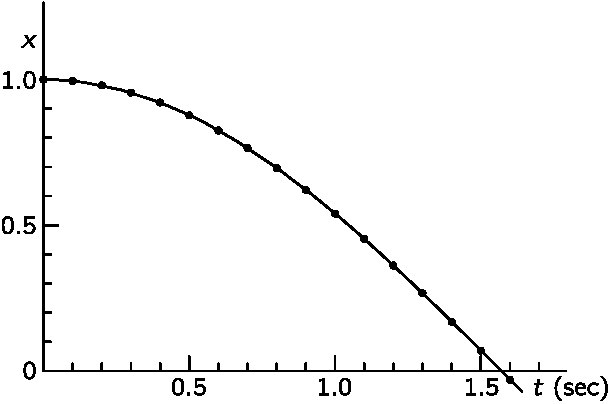
\includegraphics[width=0.6\linewidth]{fyz_fig102.pdf}
      \caption{Graf pohybu závaží na pružině (\cite[s.~129]{Feynman01})}
      \label{fyz:fig102}
    \end{figure}
    
    Tabulka nám poskytuje velmi dobrou představu o pohybu: Pohyb začíná z klidu, pak závaží získává 
    malou rychlost směrem nahoru (zápornou) a zmenšuje se vzdálenost od rovnovážné polohy. 
    Zrychlení je pak sice trochu menší, ale ještě stále se zvyšuje rychlost. Rychlost se však 
    zvyšuje stále méně a méně, až při přechodu bodem \(x = 0\) přibližně v čase \(t = 
    \SI{1.5}{\s}\) dojde k opačnému pohybu: poloha \(x\) bude záporná a zrychlení tedy kladné. 
    Rychlost se zmenšuje. Bude zajímavé porovnat údaje v tabulce s funkcí \(x = \cos t\). Takové 
    porovnání najdeme na obr. \ref{fyz:fig102}. Je vidět shoda s našimi výpočty s přesností na tři 
    platné číslice! Později uvidíme, že \(x = \cos t\) je přesné matematické řešení naší pohybové 
    rovnice. Uvedený postup ukazuje sílu numerické analýzy, která takovým jednoduchým výpočtem 
    poskytla přesné výsledky.
    
    \begin{table}[ht!]      %\ref{fyz:tab006}
      \centering
      \scalebox{0.8}{
      \begin{tabular}{|>{\centering\arraybackslash}p{3em}|>{\centering\arraybackslash}p{4em}
                      |>{\centering\arraybackslash}p{4em}|>{\centering\arraybackslash}p{4em}|}
        \hline  
         \(t\) & \(x\) & \(v_x\)  & \(a_x\)     \\
        \hline
           \num{0.0} &  \num{1.000} & \multirow{2}{*}{\num{-0.050}} & \num{-1.000} \\ 
           \num{0.1} &  \num{0.995} & \multirow{2}{*}{\num{-0.150}} & \num{-0.995} \\
           \num{0.2} &  \num{0.980} & \multirow{2}{*}{\num{-0.248}} & \num{-0.980} \\
           \num{0.3} &  \num{0.955} & \multirow{2}{*}{\num{-0.343}} & \num{-0.955} \\
           \num{0.4} &  \num{0.921} & \multirow{2}{*}{\num{-0.435}} & \num{-0.921} \\
           \num{0.5} &  \num{0.877} & \multirow{2}{*}{\num{-0.523}} & \num{-0.877} \\
           \num{0.6} &  \num{0.825} & \multirow{2}{*}{\num{-0.605}} & \num{-0.825} \\
           \num{0.7} &  \num{0.764} & \multirow{2}{*}{\num{-0.682}} & \num{-0.764} \\
           \num{0.8} &  \num{0.696} & \multirow{2}{*}{\num{-0.751}} & \num{-0.695} \\
           \num{0.9} &  \num{0.621} & \multirow{2}{*}{\num{-0.814}} & \num{-0.621} \\
           \num{1.0} &  \num{0.540} & \multirow{2}{*}{\num{-0.868}} & \num{-0.540} \\
           \num{1.1} &  \num{0.453} & \multirow{2}{*}{\num{-0.913}} & \num{-0.453} \\
           \num{1.2} &  \num{0.362} & \multirow{2}{*}{\num{-0.949}} & \num{-0.362} \\
           \num{1.3} &  \num{0.267} & \multirow{2}{*}{\num{-0.976}} & \num{-0.267} \\
           \num{1.4} &  \num{0.169} & \multirow{2}{*}{\num{-0.993}} & \num{-0.169} \\
           \num{1.5} &  \num{0.070} & \multirow{2}{*}{\num{-1.000}} & \num{-0.070} \\
           \num{1.6} & \num{-0.030} &                               & \num{-0.030} \\
        \hline 
      \end{tabular}}
      \caption{Řešení rovnice \(\der{v_x}{t} = -x\), interval \(\varepsilon = \SI{0.1}{\s}\)  
               (\cite[s.~130]{Feynman01})}
      \label{fyz:tab006}
     \end{table}

  \section{Pohyb planet}\label{fyz:IchapIXsecVII}
    Předcházející analýza je velmi vhodná k popisu kmitající stru\-ny. Nás však zajímá, zda je 
    takto 
    možné analyzovat i pohyb planet kolem Slunce. Zjistíme, je-li možné v jistém přiblížení dospět 
    k eliptické oběžné dráze. Budeme předpokládat, že Slunce je nekonečně těžké v tom smyslu, že 
    nemusíme uvažovat jeho pohyb. Dále předpokládejme, že planeta začala svůj pohyb na určitém 
    místě a pohybuje se určitou rychlostí kolem Slunce po nějaké křivce. Pomocí Newtonových 
    pohybových zákonů a gravitačního zákona se pokusíme zjistit, jaká je to křivka. Jak to 
    provedeme? V daném okamžiku je planeta v určitém bodě v prostoru. Označíme-li \(r\) radiální 
    vzdálenost od Slunce k tomuto bodu, pak víme, že na planetu působí síla směřující ke Slunci, 
    která je podle gravitačního zákona rovna konstantě násobené součinem hmotností Slunce a planety 
    a dělené druhou mocninou jejich vzdálenosti. K dalším úvahám potřebujeme vědět, jaké zrychlení 
    vyvolává tato síla. Potřebujeme znát složky zrychlení ve dvou směrech, jimiž vedeme osy \(x\) a 
    \(y\) (počátek umístíme v Slunci). Poloha planety v daném okamžiku je určena souřadnicemi \(x\) 
    a \(y\) (o souřadnici \(z\) předpokládáme, že je stále nulová, neboť v tom směru nepůsobí žádná 
    síla, a jestliže počáteční rychlost \(v_z\) byla nulová, není důvod, aby se souřadnice 
    změnila). Gravitační síla směřuje podél spojnice planety a Slunce, jak je vidět na obr. 
    \ref{fyz:fig103}.

    \luagraphic[0.8]{fyz_fig103.pdf}{Gravitační síla působící na planetu 
    (\cite[s.~131]{Feynman01})}{fyz:fig103}

    Z uvedeného obrázku je vidět, že horizontální složka síly souvisí s celkovou silou stejným 
    způsobem, jakým horizontální souřadnice \(x\) souvisí s celkovou délkou přepony \(r\), neboť 
    příslušné trojúhelníky jsou podobné. Dále, je-li \(x\) kladné, bude \(F_x\) záporné. Je \(F_x = 
    -\abs{F}x/r\), tedy \(F_x = -\abs{F}x/r = -\kappa Mmx/r^3\). Využijme nyní dynamického zákona 
    (\ref{fyz:eq063}), z něhož vyplývá, že \(x\)-ová nebo \(y\)-ová složka zrychlení násobená 
    hmotností planety je rovna \(x\)-ové resp. \(y\)-ové složce síly. Tak dostaneme rovnice
    \begin{subequations}\label{fyz:eq133}
      \begin{align} 
        m\left(\der{v_x}{t}\right) &= -\frac{\kappa Mmx}{r^3}, \label{fyz:eq133a}   \\
        m\left(\der{v_y}{t}\right) &= -\frac{\kappa Mmy}{r^3}, \label{fyz:eq133b}   \\
                                r &= \sqrt{x^2+y^2}.          \label{fyz:eq133c} 
      \end{align}
    \end{subequations}
    
    Tuto soustavu rovnic musíme řešit. Abychom si zjednodušili numerický výpočet, budeme opět 
    předpokládat, že jednotka času nebo hmotnost Slunce jsou vybrány tak (nebo máme takové štěstí), 
    že \(\kappa M = 1\). V našem případě budeme předpokládat, že počáteční poloha planety je \(x= 
    0,500\), \(y = 0,000\) a počáteční rychlost je ve směru osy \(y\) a je rovna \num{1.6300}. Jak 
    provedeme výpočet? Opět si sestavíme tabulku se sloupci pro čas, \(x\)-ovou souřadnici, 
    \(x\)-ovou složku rychlosti \(v\) a \(x\)-ovou složku zrychlení \(a_x\); pak následují tři 
    sloupce oddělené dvojitou čarou pro souřadnici, rychlost a zrychlení v \(y\)-ovém směru. K 
    získání zrychlení budeme potřebovat rovnice (9.17), z nichž zjistíme, že zrychlení má složky 
    \(-x/r^3\) a \(-y/r^3\), přičemž \(r=\sqrt{x^2 + y^2}\). Známe-li tedy hodnoty \(x\) a \(y\), 
    musíme někde stranou provést malý výpočet, tj. najít odmocninu ze součtu druhých mocnin, tak 
    najít \(r\) a pak počítat příslušná zrychlení. Je užitečné určit i \(1/r^3\). Takovýto výpočet 
    je poměrně jednoduchý - stačí použít tabulku druhých a třetích mocnin a převrácených hodnot; 
    pak už potřebujeme jen \(x\) násobit \(1/r^3\).
    
    Postup našeho výpočtu je pak následující: Zvolíme si časový interval \(\varepsilon = 
    \num{0.100}\). Počáteční hodnoty v čase \(t = 0\) jsou
    \begin{align*}
      x(0)    &= \num{0.500}  \quad y(0) = \num{0.000}                                \\
      v_x(0)  &= \num{0.000}  \quad v_y(0) = \num{1.630}                              \\
      \shortintertext{Odtud najdeme}
      r(0)    &= \num{0.500}  \quad \frac{1}{r^3}(0) = \num{8.000}                    \\
      a_x     &= \num{-4.000} \quad a_y = \num{0.000}
      \shortintertext{Pak můžeme vypočítat složky 
                      rychlosti \(v_x(\num{0.05}\) a \(v_x(\num{0.05})\)}              
      v_x(\num{0.05}) &= 0,000 - 4,000\cdot0,050 = \num{-0.200}                        \\
      v_y(\num{0.05}) &= 1,630 + 0,000\cdot0,050 = \num{1.630}                         \\
      \shortintertext{Nyní začíná náš hlavní výpočet}
      x(0,1) &= \num{0.500} - \num{0.20}\cdot\num{0.1} = \num{0.480}                   \\
      y(0,1) &= \num{0.0}   - \num{1.63}\cdot\num{0.1} = \num{0.163}                   \\
          r  &= \sqrt{\num{0.480}^2 + \num{0.163}^2} = \num{0.507}                     \\
      \frac{1}{r^3}   &= \num{7.67}                                                    \\
      a_x(0,1)  &= \num{-0.480}\cdot\num{7.67} = \num{-3.68}                           \\
      a_y(0,1)  &= \num{-0.163}\cdot\num{7.67} = \num{-1.256}                          \\
      v_x(0,15) &= \num{-0.200} \num{-3.68}\cdot\num{0.1} = \num{-0.568}               \\
      v_y(0,15) &= \num{1.630} \num{-1.26}\cdot\num{0.1} = \num{-1.505}                \\
      x(0,2)    &= \num{0.480} \num{-0.568}\cdot\num{0.1} = \num{0.423}                \\
      y(0,2)    &= \num{0.163} \num{1.50}  \cdot\num{0.1} = \num{0.313} \quad\text{atd.}    
    \end{align*}
    
    
    Takovým způsobem získáme hodnoty uvedené v tab. \ref{fyz:tab001} a přibližné ve dvaceti krokách 
    vystopujeme polovinu dráhy planety kolem Slunce. Na obr. \ref{fyz:fig103} jsou zakresleny 
    \(x\)-ové a \(y\)-ové souřadnice z tab. \ref{fyz:tab001}. Tečky představují polohy v 
    posloupnosti časů vzdálených o desetinu zvolené časové jednotky. Je vidět, že na počátku se 
    planeta pohybuje rychleji, na konci pomaleji a je zřejmý i tvar křivky. Vidíme tedy, že opravdu 
    umíme počítat pohyb planet!

    
    \begin{table*}[ht!]      %\ref{fyz:tab001}
      \centering
      \scalebox{0.7}{
      \begin{tabular}{ |>{\centering\arraybackslash}p{3em}||>{\centering\arraybackslash}p{4em}
                        |>{\centering\arraybackslash}p{4em}|>{\centering\arraybackslash}p{4em}
                        ||>{\centering\arraybackslash}p{4em}|>{\centering\arraybackslash}p{4em}
                        |>{\centering\arraybackslash}p{4em}||>{\centering\arraybackslash}p{4em}
                        |>{\centering\arraybackslash}p{4em}|}
        \hline 
        \(t\)  & \(x\) & \(v_x\) & \(a_x\) & \(y\) & \(v_y\) &  \(a_y\) & \(r\) & \(1/r^3\) \\ 
        \hline      
        \num{0.0} & \num{+0.500} & \multirow{2}{*}{\num{-0.200}} & \num{-4.000} & \num{+0.000} & 
        \multirow{2}{*}{\num{+1.630}} & \num{+0.00} & \num{0.500} & \num{8.500} \\  
        \num{0.1} & \num{+0.480} & \multirow{2}{*}{\num{-0.568}} & \num{-3.680} & \num{+0.163} & 
        \multirow{2}{*}{\num{+1.505}} & \num{-1.25} & \num{0.507} & \num{7.675} \\  
        \num{0.2} & \num{+0.423} & \multirow{2}{*}{\num{-0.859}} & \num{-2.910} & \num{+0.313} & 
        \multirow{2}{*}{\num{+1.290}} & \num{-2.15} & \num{0.526} & \num{6.873} \\  
        \num{0.3} & \num{+0.337} & \multirow{2}{*}{\num{-1.055}} & \num{-1.960} & \num{+0.442} & 
        \multirow{2}{*}{\num{+1.033}} & \num{-2.57} & \num{0.556} & \num{5.824} \\  
        \num{0.4} & \num{+0.232} & \multirow{2}{*}{\num{-1.116}} & \num{-1.110} & \num{+0.545} & 
        \multirow{2}{*}{\num{+0.771}} & \num{-2.62} & \num{0.592} & \num{4.810} \\  
        \num{0.5} & \num{+0.115} & \multirow{2}{*}{\num{-1.211}} & \num{-0.453} & \num{+0.622} & 
        \multirow{2}{*}{\num{+0.526}} & \num{-2.45} & \num{0.633} & \num{3.942} \\  
        \num{0.6} & \num{-0.006} & \multirow{2}{*}{\num{-1.209}} & \num{+0.020} & \num{+0.675} & 
        \multirow{2}{*}{\num{+0.306}} & \num{-2.20} & \num{0.675} & \num{3.252} \\  
        \num{0.7} & \num{-0.127} & \multirow{2}{*}{\num{-1.175}} & \num{+0.344} & \num{+0.706} & 
        \multirow{2}{*}{\num{+0.115}} & \num{-1.91} & \num{0.717} & \num{2.712} \\  
        \num{0.8} & \num{-0.245} & \multirow{2}{*}{\num{-1.119}} & \num{+0.562} & \num{+0.718} & 
        \multirow{2}{*}{\num{-0.049}} & \num{-1.64} & \num{0.758} & \num{2.296} \\  
        \num{0.9} & \num{-0.357} & \multirow{2}{*}{\num{-1.048}} & \num{+0.705} & \num{+0.713} & 
        \multirow{2}{*}{\num{-0.190}} & \num{-1.41} & \num{0.797} & \num{1.975} \\  
        \num{1.0} & \num{-0.462} & \multirow{2}{*}{\num{-0.968}} & \num{+0.796} & \num{+0.694} & 
        \multirow{2}{*}{\num{-0.310}} & \num{-1.20} & \num{0.834} & \num{1.723} \\  
        \num{1.1} & \num{-0.559} & \multirow{2}{*}{\num{-0.882}} & \num{+0.858} & \num{+0.663} & 
        \multirow{2}{*}{\num{-0.412}} & \num{-1.02} & \num{0.867} & \num{1.535} \\  
        \num{1.2} & \num{-0.647} & \multirow{2}{*}{\num{-0.792}} & \num{+0.900} & \num{+0.622} & 
        \multirow{2}{*}{\num{-0.499}} & \num{-0.86} & \num{0.897} & \num{1.385} \\  
        \num{1.3} & \num{-0.726} & \multirow{2}{*}{\num{-0.700}} & \num{+0.920} & \num{+0.572} & 
        \multirow{2}{*}{\num{-0.570}} & \num{-0.72} & \num{0.924} & \num{1.267} \\  
        \num{1.4} & \num{-0.796} & \multirow{2}{*}{\num{-0.607}} & \num{+0.930} & \num{+0.515} & 
        \multirow{2}{*}{\num{-0.630}} & \num{-0.60} & \num{0.948} & \num{1.173} \\  
        \num{1.5} & \num{-0.857} & \multirow{2}{*}{\num{-0.513}} & \num{+0.940} & \num{+0.452} & 
        \multirow{2}{*}{\num{-0.680}} & \num{-0.50} & \num{0.969} & \num{1.099} \\  
        \num{1.6} & \num{-0.908} & \multirow{2}{*}{\num{-0.418}} & \num{+0.950} & \num{+0.384} & 
        \multirow{2}{*}{\num{-0.720}} & \num{-0.40} & \num{0.986} & \num{1.043} \\  
        \num{1.7} & \num{-0.950} & \multirow{2}{*}{\num{-0.323}} & \num{+0.950} & \num{+0.312} & 
        \multirow{2}{*}{\num{-0.751}} & \num{-0.31} & \num{1.000} & \num{1.000} \\  
        \num{1.8} & \num{-0.982} & \multirow{2}{*}{\num{-0.288}} & \num{+0.950} & \num{+0.237} & 
        \multirow{2}{*}{\num{-0.773}} & \num{-0.23} & \num{1.010} & \num{0.970} \\  
        \num{1.9} & \num{-1.005} & \multirow{2}{*}{\num{-0.113}} & \num{+0.950} & \num{+0.160} & 
        \multirow{2}{*}{\num{-0.778}} & \num{-0.15} & \num{1.018} & \num{0.948} \\  
        \num{2.0} & \num{-1.018} & \multirow{2}{*}{\num{-0.037}} & \num{+0.960} & \num{+0.081} & 
        \multirow{2}{*}{\num{-0.796}} & \num{-0.08} & \num{1.021} & \num{0.939} \\  
        \num{2.1} & \num{-1.022} & \multirow{2}{*}{\num{0.058}}  & \num{+0.950} & \num{+0.001} & 
        \multirow{2}{*}{\num{-0.796}} & \num{-0.00} & \num{1.022} & \num{0.936} \\  
        \num{2.2} & \num{-1.016} &                               & \num{+0.960} & \num{-0.079} & 
        \multirow{2}{*}{\num{-0.789}} & \num{-0.07} & \num{1.019} & \num{0.945} \\  
        \num{2.3} &              &                               &              &              
        &                               &             &             &             \\  
        \hline 
      \end{tabular}}
      \caption{Řešení soustavy rovnic \(\der{v_x}{t} = -\frac{x}{r^3}\); \(\der{v_y}{t} = 
               -\frac{y}{r^3}\); \(r = \sqrt{x^2 + y^2}\); interval: \(\varepsilon = \num{0.100}\); 
               Orbita \(v_y = \num{1.63}\), \(v_x = \num{0}\), \(x = \num{0.5}\), \(y = \num{0}\) v 
               okamžiku \(t = 0\)}
      \label{fyz:tab001}
    \end{table*}
   
    Trajektorie protíná osu \(x\) v okamžiku \(t = \SI{2.101}{\s}\); perioda oběhu je 
    \SI{4.20}{\s}; \(v_x = 0\) v okamžiku \(t = \SI{2.086}{\s}\). Trajektorie vytíná na ose \(x\) 
    úsek \(x= \num{1.022}\); délka hlavní poloosy je rovna \((\num{1.022} + \num{0.500})/2 = 
    \num{0.761}\); \(v_y = \num{0,796}\). Předpovídaná doba polovičního oběhu 
    \(\pi(\num{0.761})^{3/2} = \pi(\num{0.663}) = \num{2.082}\).
    
    Nyní si ukážeme, jak je možné vypočítat pohyb Neptunu, Jupiteru, Uranu nebo kterékoli jiné 
    planety. Je možno provést výpočty pro velké množství planet, bereme-li v úvahu i pohyb Slunce? 
    Samozřejmě, že ano. Vypočítáme sílu působící na zvolenou planetu, např. na \(i\)-tou planetu, 
    jež má polohu \(x_i, y_i, z_i\) (\(i = 1\) může představovat Slunce, \(i = 2\) Merkur, \(i = 
    3\) Venuši atd.). Musíme znát polohy všech planet. Síla působící na jednu planetu je výsledkem 
    vlivu všech ostatních těles, která se nacházejí v polohách \(x_j, y_j, z_j\) .Tak získáme 
    rovnice.
    \begin{subequations}
      \label{fyz:eq134}
      \begin{align}
        m_i\der{v_{ix}}{t} 
          &= \sum_{j=1}^N - \frac{\kappa M_im_j(x_i - x_j)}{r_{ij}^3}  \label{fyz:eq134a}  \\
        m_i\der{v_{iy}}{t} 
          &= \sum_{j=1}^N - \frac{\kappa M_im_j(y_i - y_j)}{r_{ij}^3}  \label{fyz:eq134b}  \\
        m_i\der{v_{iz}}{t} 
          &= \sum_{j=1}^N - \frac{\kappa M_im_j(z_i - z_j)}{r_{ij}^3}  \label{fyz:eq134c}  
      \end{align}
    \end{subequations}
    Pod \(r_{ij}\) rozumíme vzdálenost mezi dvěma planetami \(i\) a \(j\)
    \begin{equation}\label{fyz:eq135}
      r_{ij} = \sqrt{(x_i-x_j)^2 + (y_i-y_j)^2 + (z_i-z_j)^2}
    \end{equation}
    
    Symbol \(\sum\) označuje součet přes všechny hodnoty \(j\)-všechna ostatní tělesa, samozřejmě 
    kromě \(j = i\). Všechno, co musíme udělat, je vytvořit \emph{mnohem} více sloupců. Potřebujeme 
    devět sloupců pro pohyb Jupiteru, devět pro pohyb Saturnu atd. Jsou-li dány všechny počáteční 
    polohy a rychlosti, můžeme z rovnic (\ref{fyz:eq134}) vypočítat všechna zrychlení, přičemž 
    nejdříve pomocí vztahu (\ref{fyz:eq135}) vypočteme všechny vzdálenosti. Jak dlouho nám takový 
    výpočet potrvá? Budeme-li ho provádět doma, zabere velmi mnoho času. Dnes však máme stroje, jež 
    to provedou velmi rychle.
    
    \begin{figure}[ht!]  %\ref{fyz:fig104}
      \centering
      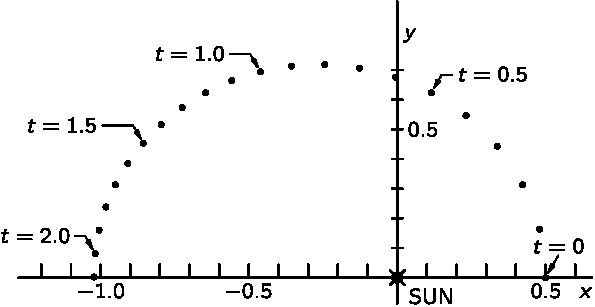
\includegraphics[width=0.7\linewidth]{fyz_fig104.pdf}
      \caption{Vypočítaný pohyb planety kolem Slunce (\cite[s.~134]{Feynman01})}
      \label{fyz:fig104}
    \end{figure}
    
    Kdyby počítači trvalo sčítání \SI{1}{\us}, násobení asi \SI{10}{\us}. Bude-li v 
    jednom výpočetním cyklu nějaké úlohy například \num{30} násobení, pak takový cyklus potrvá 
    \SI{300}{\us}. Pak můžeme za jednu sekundu provést \num{3000} výpočetních cyklů. Kdybychom 
    chtěli pracovat s přesností na jednu miliardtinu, potřebovali bychom \num{4e5} cyklů k pokrytí 
    jednoho oběhu planety kolem Slunce. To odpovídá výpočetnímu času 130 sekund, tedy asi dvěma 
    minutám. Touto metodou tedy můžeme vypočítat pohyb Jupiteru kolem Slunce s přesností na 
    jednu miliardtinu při uvážení vlivu všech ostatních planet za pouhé dvě minuty! (Ukazuje se, že 
    chyba ve výpočtech je přibližně úměrná druhé mocnině intervalů \(\varepsilon\). Zmenšíme-li 
    interval na tisícinu, zvětší se přesnost miliónkrát. Pro zajištění námi požadované přesnosti 
    musíme vzít interval \num{10000}-krát menší.)
    
    Na začátku této kapitoly jsme nevěděli ani to, jak vypočítat pohyb závaží na pružině. Nyní, 
    vyzbrojeni takovým úžasným pomocníkem, jakým jsou Newtonovy zákony, dokážeme vypočítat nejen 
    tak jednoduchý pohyb, ale pomocí počítače, který za nás provede aritmetické výpočty, i velmi 
    složité pohyby planet s takovým stupněm přesnosti, jaký požadujeme.
    
  \section{Příklady a cvičení}
      %---------------------------------------------------------------
        % !TeX spellcheck = cs_CZ
\begin{example}Výstřel z děla (ve vakuu).
  Dělová koule opouští hlaveň zadanou rychlostí. Určete:
  \begin{itemize}[noitemsep]
    \item maximální dostřel pro zadanou úsťovou rychlost,
    \item hranice oblasti, ve kterém lze zasáhnout cíl,
    \item stanovte velikost potřebného náměru děla pro zasažení libovolného cíle uvnitř ochranné paraboly.
  \end{itemize}

  {\centering
  \luafigure[1]{fyz_fig0223a.pdf}      \\
  \luafigure[0.5]{fyz_fig0223b.pdf}
  \captionsetup{type=figure}  
  \captionof{figure}{K příkladu výpočtu trajektorie projektilu. Goniometrický vzorec
           $\vert\cos\alpha\rvert=\frac{1}{\sqrt{1+\tan\alpha^2}}$ lze snadno odvodit z náčrtu
           pomocí Pythagorovy věty (Přepona pravoúhlého trojúhelníka je $\sqrt{1+\tan\alpha^2}$)}           
  \label{fyz:fig0223}
  \par}

  \textbf{Řešení:}
  Uvažujme rovinný pohyb v rovině $xz$, přičemž v záporném směru osy $z$ má pohyb zrychlení 
  velikosti $g$. Ve směru osy $z$ tedy probíhá rovnoměrně zrychlený pohyb podle rov. 
  \ref{mech:eq_const_acc}. Vztáhneme-li počáteční podmínky k okamžiku \(t = 0\), máme
  \begin{equation}\label{mech_eq_delo_vakuum_osa_z}
    z(t)=z_0+v_{0z}t-\frac{1}{2}gt^2, \qquad v_z(t)=v_{0z}-gt
  \end{equation}
  Ve směru osy \(x\) je pohyb rovnoměrný:
  \begin{equation}\label{mech_eq_delo_vakuum_osa_x}
    x(t)=x_0+v_{0x} t,\qquad v_x(t)=v_{0x}=\mathrm{konst}
  \end{equation}

  Dělová koule opouští hlaveň pod elevačním úhlem $\alpha$ za podmínek dle obr. 
  \ref{fyz:fig0223} platí $x_0=0, z_0=0, v_{0x}=v_0\cos\alpha>0, v_{0z}=v_0\sin\alpha>0$. Jde 
  tedy o skládání \emph{rovnoměrného přímočarého pohybu s rychlostí} $v_0\cos\alpha$ ve směru osy 
  \(x\) a svislého pohybu vzhůru. Získané rovnice
  \begin{equation}\label{mech:eq_delo_rce_pohybu}
    z(t)=v_{0z}t-\frac{1}{2}gt^2, \qquad x(t)=v_{0x}t
  \end{equation}
  představují \emph{parametrické rovnice trajektorie}. Vyloučíme-li z nich čas $t$, dostaneme 
  rovnici křivky v kartézských souřadnicích
  \begin{equation}\label{mech:eq_delo_vakuum_param_rce}
    z(x)=  \frac{v_{0z}}{v_{0x}}x-\frac{1}{2}\frac{g}{v_{0x}^2}x^2
        = x\tan\alpha-\frac{1}{2}\frac{g}{v_0^2\cos^2\alpha}x^2
  \end{equation}
  Nyní aplikujeme goniometrický vzorec
  \begin{equation*}
    \vert\cos\alpha\rvert = \frac{1}{\sqrt{1+\tan^2\alpha}}\Rightarrow \frac{1}{\cos^2\alpha} 
                          = 1+\tan^2\alpha
  \end{equation*}
  odvozený dle náčrtku na obrázku \ref{fyz:fig0223} a dostáváme rovnici
  \begin{equation}\label{mech_eq_example_vysledna_rce}
    z(x)=x\tan\alpha-\frac{1}{2}\frac{g}{v_0^2}(1+\tan^2\alpha)x^2
  \end{equation}
  Pohyb projektilu (dělové koule) probíhá po stejné trajektorii, jako šikmý vrh v homogenním 
  tíhovém poli ve vakuu, tedy po parabole. Snadno dostaneme \emph{souřadnice vrcholu dráhy, dálku 
  doletu a celkovou dobu letu}.

  \begin{itemize}
    \item Maximální dolet pro daný elevační úhel:
      \begin{equation}\label{mech:eq_elevacni_uhel_1}
        0=x\tan\alpha-\frac{1}{2}\frac{g}{v_0^2}(1+\tan^2\alpha)x^2
      \end{equation}
      \emph{Netriviální kořen této kvadratické rovnice je námi hledaný dolet dělové koule}
      \begin{align}  %\label{fyz:eq235}
        x_d &=\frac{2v_0^2\tan\alpha}{g(1+\tan^2\alpha)}(1+\tan^2\alpha)        \nonumber \\
            &=\frac{2v_0^2\sin\alpha\cos\alpha}{g}=\frac{v_0^2\sin{2\alpha}}{g} \label{fyz:eq235}
      \end{align}

    \item Celková doba letu:
      \begin{equation}\label{mech:eq_doba_letu}
        t_d=\frac{x_d}{v_{0x}} =\frac{2v_0^2\sin\alpha\cos\alpha}{gv_0\cos\alpha}
           =\frac{2v_0\sin\alpha}{g}
      \end{equation}

    \item Souřadnice vrcholu dráhy: \emph{získáme derivováním rov.
          \ref{mech_eq_example_vysledna_rce}}
          \begin{align}
            0   &= tan\alpha-\frac{g}{v_0^2(1+\tan^2\alpha)}x_v                         \\
            x_v &= \frac{v_0^2}{g}\frac{\tan\alpha}{1+\tan^2\alpha}=
                   \frac{v_0^2}{g}\frac{\sin\alpha}{\cos\alpha}
                   \cdot\cos^2\alpha\cdot\frac{2}{2}                                   \\
            x_v &= \frac{v_0^2\sin{2\alpha}}{2g}
           \end{align}
           \emph{Souřadnici $z_v$ dostaneme dosazením $x_v$  do rov.
           \ref{mech_eq_example_vysledna_rce}}
           \begin{align*}
             z_v &= \frac{v_0^2}{g}\frac{\tan^2\alpha}{1+\tan^2\alpha}-
                    \frac{1}{2}\frac{g}{v_0^2}(1+\tan^2\alpha)\frac{v_0^4}{g^2}
                    \frac{\tan^2\alpha}{(1+\tan^2\alpha)^2}                            \\
             z_v &= \frac{v_0^2}{g}\frac{\tan^2\alpha}{1+\tan^2\alpha}-
                    \frac{1}{2}\frac{v_0^2}{g}\frac{\tan^2\alpha}{1+\tan^2\alpha}      \\
             z_v &= \frac{v_0^2\sin^2\alpha}{2g}
      \end{align*}
      \emph{Odtud je zřejmé, že maximální délka doletu odpovídá úhlu $\frac{\pi}{4}$ a že obecně 
      daného bodu doletu lze dosáhnout pod dvěma různými úhly $\frac{\pi}{4}\pm\Delta\alpha$.}

    \item Stanovení elevačního úhlu pro zasažení zadaných souřadnic $[X_c, Z_c]$ cíle: \emph{Opět  
          vycházíme z rov. \ref{mech_eq_example_vysledna_rce}, ovšem tentokrát nejsou neznáme \(x\) a 
          $z$, ale $\alpha$: Použijeme substituci $\tan\alpha=p$ a vypočítáme kořeny této 
          kvadratické rovnice:}
          \begin{align}
            0       &= gx^2p^2-2v_0^2xp+(gx^2+2zv_0^2) \\
            p_{1,2} &= \frac{v_0^2\pm\sqrt{v_0^4-g(gx^2+2zv_0^2)}}{gx} \\
            \alpha  &= \tan^{-1}\left(\frac{v_0^2\pm\sqrt{v_0^4-g(gx^2+2zv_0^2)}}{gx}\right)
          \end{align}
          \emph{Je-li cíl zadán v polárních souřadnicích $[r,\varphi]$, lze potřebný náměr stanovit takto:}
          \begin{equation*}
            \alpha=\tan^{-1}\left(\frac{v_0^2\pm
                   \sqrt{v_0^4-g(gr^2\cos^2\varphi+2r\sin\varphi
                         v_0^2)}}{gr\cos\varphi}\right)
          \end{equation*}
          \emph{Pokud ovšem bude diskriminant menší než 0, leží cíl mimo dosah děla. Tj. neexistuje 
          takový náměr děla, kterým by bylo možné cíl zasáhnout. Je-li diskriminant roven nule, 
          jedná se o hranici, za kterou již při dané úsťové rychlosti nelze dostřelit. Body ležící 
          na této obálce tzv. ochranná parabola mohou být zasaženy pouze při jedné hodnotě 
          elevačního úhlu.}

    \item Stanovení rovnice ochranné paraboly: \emph{To provedeme tak, že položíme diskriminant 	
          rovnice pro $\tan\alpha$ roven nule a dostaneme rovnici obálky}
          \begin{equation}\label{mech:eq_ochr_parabola}
            v_0^4-g(gx^2+2zv_0^2)\Rightarrow z=-\frac{v_0^2}{2g^2}x^2+\frac{v_0^2}{2g}
          \end{equation}
  \end{itemize}

  %--------------------------Dělo---------------------------------
    \lstinputlisting[%
      style=luaMatlabStyle, 
      caption={\texttt{kinematika\_delo\_ve\_vakuu.m} pro ověření výpočtu balistické dráhy 
               projektilu.}
    ]{../src/FYZ/matlab/kinematika_delo_ve_vakuu.m}
  %---------------------------------------------------------------

  {\centering
    \captionsetup{type=figure}
    \luafigure[1]{fyz_fig0222.pdf}
    \captionof{figure}{Výpočet trajektorie projektilu ve vakuu při úsťové rychlosti $210 m/s$ 
              pomocí sw MATLAB\textsuperscript{\textregistered}.}
    \label{mech:fig_delo_matlab}
  \par}
\end{example}
      %---------------------------------------------------------------

%} %tikzset
%---------------------------------------------------------------------------------------------------